\documentclass[12pt]{article}
\usepackage[utf8]{inputenc}
\usepackage{graphicx}
\usepackage[style=numeric]{biblatex}
\usepackage[brazil]{babel}
\usepackage{url}
\addbibresource{ref.bib}
 
 
\title{Aprendizagem de Máquina - IF699}
\author{Matheus Braga de Britto}
\date{Maio, 2022 }
 
\begin{document}
 
\maketitle
 
\begin{figure}[h]
    \centering


    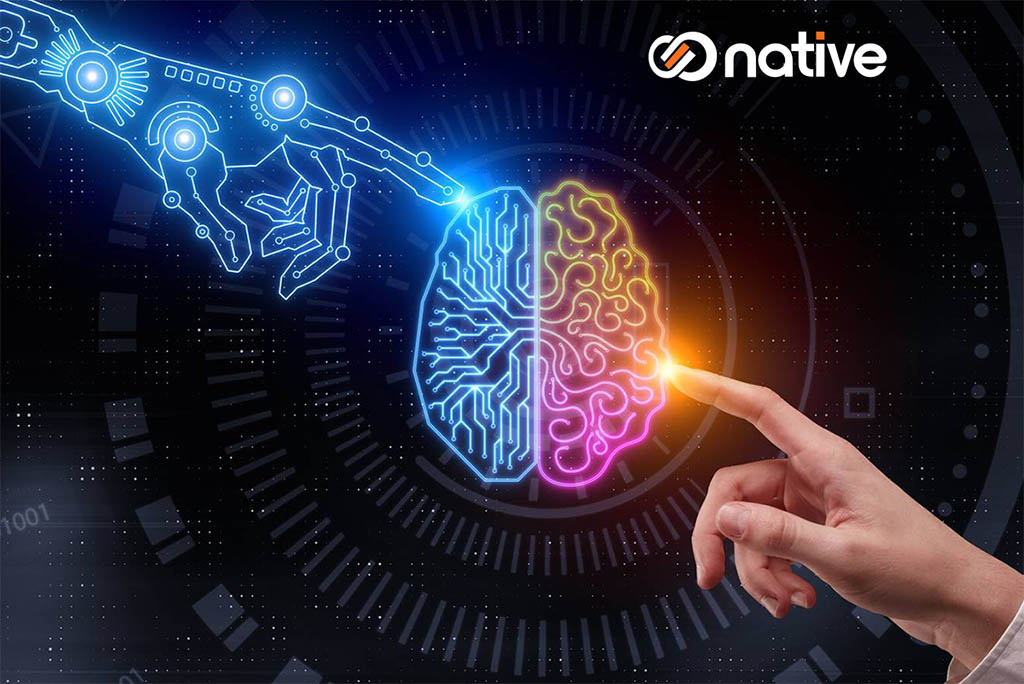
\includegraphics[width=90mm]{foto.jpg}
    \caption{Ilustração Inteligência Artificial}


\end{figure}
 
\section{Introdução}

\par 
Segundo Arthur Samuel, um programador renomado do jogo Damas, aprendizado de máquina nada mais é do que a habilidade de um computador de aprender a realizar uma tarefa sem que seja atribuida a ele uma programação explicícita, desse modo o sistema é obrigado a aprender de forma autonoma para que consiga realizar a tarefa que a ele foi solicitada.

 \cite{mahesh2020machine}

\section{Métodos e Aplicações}
\par
No Aprendizado de Máquina não há um modo certo e errado de se realizar uma tarefa, mas sim, mais ou menos otimizado. O modo mais comum utilizado para o “machine learning” é o “Supervised Learning” ou aprendizado supervisionado, nesse método, é dada à máquina uma sequência de inputs e outputs, desse modo ele conseguirá aprender qual é o output mais provável naquela situação devido a análise de padrões feitas anteriormente por ele mesmo. Devido a sua alta taxa de acerto quando se trata de padrões, o mesmo é amplamente utilizado em detecção de fraudes, análise de risco, previsão de falhas, data science, entre diversas outras aplicações práticas.


\cite{mahesh2020machine}
\cite{monard2003conceitos}


\section{Relações com outras disciplinas}
\par
A disciplina de Aprendizagem de Máquina do Cin (IF699) apresenta um curso bem completo voltado para seu propósito. Ademais, a disciplina se torna dependente da disciplina de Gerenciamento de Dados e Informação (IF685) devido ao seu alto grau de complexidade e especificidade quanto ao conteúdo exposto no curso. Este curso, contudo possui alto grau de conexão com outras disciplinas e áreas de conhecimento como por exemplo Ciência de Dados e Inteligência Artificial
\cite{de2020smart}

\printbibliography

\end{document}
